\label{ch:unfolding_methods}

To perform anomaly detection on the core, we need to apply neutron noise unfolding methods. Unfolding methods in this case are used to determine the parameters of neutron noise sources, including their magnitude, frequency, energy, and location. Neutron noise unfolding methods have been developed in the past and verified for the absorber of variable strength-type noise source, mainly light water reactor cores \cite{karlssonLocalizationChannelInstability1999, demaziereDevelopmentNonintrusiveMethod2002, demaziereIdentificationLocalizationAbsorbers2005}. The methods are the inversion method, zoning method, and scanning method. The methods rely on the use of Green’s function, which can be pre-calculated without the need to know the true neutron noise source in the core.

This chapter introduces two novel neutron noise unfolding methods based on Green’s function. These methods are called the brute force method and the greedy method. One more method, called the backward elimination method, has also been developed. However, this method is not reliable for multiple noise sources. The details for the backward elimination method are available in Appendix \ref{ch:appendixB}. For the sake of completeness, this chapter also outlines the derivation of existing neutron noise unfolding methods. These methods are used as a comparison of the new methods for HTTR core application.

The structure of this chapter is as follows. First, we will provide the derivation of Green’s function for neutron noise unfolding methods. In here, we will provide the derivation of the neutron noise as a function of the Green’s function. Second, we will provide the existing neutron noise unfolding methods and their derivations. Third, we will introduce novel neutron noise unfolding methods, their derivation and computational algorithm. Fourth, we will apply all the neutron noise unfolding methods to the 2D and 3D HTTR core. In these cases, the AVS-type noise source is used for practicality. Finally, we will provide the limitations of the novel methods and the conclusion of the chapter.

\section{Green's Function for Neutron Noise Unfolding}

Neutron noise source unfolding is a method used to identify the type of noise source and locate the position at which perturbations occur. Generally, the noise source unfolding method depends on Green’s function. Hence, determining Green’s function from the neutron noise equation is necessary \cite{demaziereIdentificationLocalizationAbsorbers2005}. We begin with the definition of the neutron noise equation in operator form.
\begin{equation}
    B(\textbf{r}) \delta \phi(\textbf{r},\omega) = S(\textbf{r},\omega)
\end{equation}
where $B(\textbf{r})$ is the Boltzmann-like operator for the complex neutron noise equation and $S(\textbf{r},\omega)$ is the neutron noise source term. Since neutron noise can be described as a localized (impulse-like) perturbation, we define Green's function of $B(\textbf{r})$ to be the unique solution of Eq. \ref{eq:Green_function1}.
\begin{equation}\label{eq:Green_function1} 
    B(\textbf{r}) G(\textbf{r}, \textbf{r}_p,\omega) = \delta(\textbf{r}-\textbf{r}_p)
\end{equation}
Then, we can define,
\begin{equation}\label{eq:greens_function}
    \delta \phi(\textbf{r}, \omega) = \int_{V_p} G(\textbf{r}, \textbf{r}_p,\omega) S(\textbf{r}_p,\omega) dV_p
\end{equation}
where
\begin{itemize}
    \item[] $\delta \phi(\textbf{r}, \omega) $ = Neutron noise,
    \item[] $G(\textbf{r}, \textbf{r}_p,\omega)$ = Green's function matrix,
    \item[] $S(\textbf{r}_p,\omega)$ = Neutron noise sources to be unfolded.
\end{itemize}

In finite mesh, Eq. \ref{eq:greens_function} can be discretized and be written as matrix-vector multiplication:
\begin{equation}
    \delta \phi(\textbf{r}, \omega) = G(\textbf{r}, \textbf{r}_p,\omega) S(\textbf{r}_p,\omega)
\end{equation}
Therefore, the noise source can be determined by inverting the Green’s function such that:
\begin{equation}\label{eq:source_initial}
    S(\textbf{r}_p,\omega) = G^{-1}(\textbf{r}, \textbf{r}_p,\omega) \delta \phi(\textbf{r}, \omega)
\end{equation}

Suppose the neutron noise is known at every location in the core. In that case, it is trivial to obtain the neutron noise source information, including the magnitude and location, by inverting the Green’s function matrix. However, this is not the case due to the limitation of detector locations. This means that Eq. \ref{eq:source_initial} should be written as:
\begin{equation}\label{eq:source_meas}
    S(\textbf{r}_p,\omega) = G^{-1}(\textbf{r}_{\text{meas}}, \textbf{r}_p,\omega) \delta \phi(\textbf{r}_{\text{meas}}, \omega)
\end{equation}
where $\delta \phi(\textbf{r}_{\text{meas}}, \omega)$ means that the neutron noise is known at detector locations (measured) and zero otherwise. This creates a non-square matrix for the Green’s function, which makes it ill-posed to invert. This is the main challenge of neutron noise unfolding methods.

\section{Existing Neutron Noise Unfolding Methods}

\subsection{Inversion Method}

Inversion method is proposed by \cite{demaziereIdentificationLocalizationAbsorbers2005} to unfold the neutron noise sources by interpolating the detector readings to match the vector size $\delta \phi (\textbf{r}, \omega)$. The study assumes that the detector is sensitive to thermal neutron and the noise source is known to be a perturbation of thermal absorption cross-section \cite{demaziereIdentificationLocalizationAbsorbers2005}. The interpolated neutron noise $\delta \phi (\textbf{r}_{\text{interp}}, \omega)$ can be written as follows:
\begin{equation}
    \begin{aligned}
        \delta \phi (\textbf{r}_{\text{interp}}, \omega) &= \overline{\overline{T}} \delta \phi (\textbf{r}, \omega) \\
        &= \overline{\overline{T}} G(\textbf{r}, \textbf{r}_p,\omega) S(\textbf{r}_p,\omega) \\
        &= G(\textbf{r}_{\text{interp}}, \textbf{r}_p,\omega) S(\textbf{r}_p,\omega)
    \end{aligned}
\end{equation}
Therefore, the neutron noise source is written as:
\begin{equation}
    S(\textbf{r}_p,\omega) = G^{-1}(\textbf{r}_{\text{interp}}, \textbf{r}_p,\omega) \delta \phi (\textbf{r}_{\text{interp}}, \omega)
\end{equation}
where $\overline{\overline{T}}$ is a matrix that represents the interpolation process \cite{demaziereIdentificationLocalizationAbsorbers2005}. In this case, $G^{-1}(\textbf{r}_{\text{interp}}, \textbf{r}_p,\omega)$ has size $(\text{group} \times N), (\text{group} \times  N)$, $\delta \phi (\textbf{r}_{\text{interp}}, \omega)$ has size $\text{group} \times N$, and $S(\textbf{r}_p,\omega)$ has size $\text{group} \times N$. This means that not only the $\delta \phi (\textbf{r}, \omega)$ that needs to be interpolated, but also $G(\textbf{r}, \textbf{r}_p,\omega)$ that needs to be interpolated.

The pseudo algorithm of the inversion method is described in Algorithm~\ref{alg:inversion}.
\begin{algorithm}[H]
\caption{: Inversion Method}
\label{alg:inversion}
\begin{algorithmic}[1]
\Require Measured neutron noise $\delta \phi(\textbf{r}_{\text{meas}}, \omega)$, Green’s function matrix $G(\textbf{r}, \textbf{r}_p,\omega)$, energy groups $g$, position mesh $n$
\Ensure Reconstructed neutron noise $\delta \phi_{\text{INVERT}}(\textbf{r}, \omega)$, unfolded source $S_{\text{INVERT}}(\textbf{r}, \omega)$
\For{each group $g$} \Comment{\textbf{Interpolate $\delta \phi_{\text{meas}}$}}
    \State Collect geometry data
    \State Interpolate missing values via RBF $\rightarrow \delta \phi_{\text{INVERT}}(\textbf{r}, \omega)$
\EndFor
\For{each group $g$ and position $n$} \Comment{\textbf{Interpolate $G(\textbf{r}_{\text{meas}}, \textbf{r}_p,\omega)$}}
    \State Interpolate missing columns of $G$ $\rightarrow G(\textbf{r}_{\text{interp}}, \textbf{r}_p,\omega)$
\EndFor
\State Compute $G^{\dagger}(\textbf{r}_{\text{interp}}, \textbf{r}_p,\omega) =$ pseudo-inverse of interpolated $G$ \Comment{\textbf{Invert System}}
\State Compute unfolded sources $S_{\text{INVERT}}(\textbf{r}_p,\omega) = G^{\dagger}(\textbf{r}_{\text{interp}}, \textbf{r}_p,\omega) \delta \phi_{\text{INVERT}}(\textbf{r}, \omega)$
\State \textbf{Postprocess}: $S_{\text{INVERT}}(\textbf{r},\omega)$ file, $\delta \phi_{\text{INVERT}}(\textbf{r}, \omega)$ file, plots. 
\end{algorithmic}
\end{algorithm}

This method is able to reconstruct the noise source. However, this inversion method might have some problems in the boundaries because the interpolated thermal flux perturbation is forced to be equal to zero outside the reflector nodes. Even though the reconstruction at the boundaries produced poor approximation, the overall process still provides promising results. The result of this method is highly dependent on the interpolation process.

\subsection{Zoning Method}

The zoning method is an extension of the inversion method. The difference between the two lies in using zones in the zoning method instead of interpolation. In the zoning method, the reactor is divided into several zones, $Z_k$. Each zone has the number of detectors that is identical to the number of fuel assemblies in the zone. In this method, the flux perturbation can be written as \cite{demaziereIdentificationLocalizationAbsorbers2005}:
\begin{equation}
    \delta \phi (\textbf{r}_{\text{meas}}, \omega) = \sum_k G(\textbf{r}_{\text{meas}}, \textbf{r}_{Z_k},\omega) S(\textbf{r}_{Z_k},\omega)
\end{equation}
Since the number of detectors and the fuel assembly in the zone is identical, the Green’s function matrix $G(\textbf{r}_{\text{meas}}, \textbf{r}_{Z_k},\omega)$ for each zone is a square matrix. This means that interpolation of the Green’s function is no longer necessary.

If the fuel assemblies represented in the zone $Z_k$ are set not to be close to each other, the response of the thermal flux detector will be unique to each other. Having the fuel assemblies belonging to a given zone $Z_k$ evenly distributed throughout the core is an easy and practical way to achieve such a goal.

Then, by inverting one of the matrices $G(\textbf{r}_{\text{meas}}, \textbf{r}_{Z_k},\omega)$ for zone $Z_l$, one can obtain:
\begin{equation}\label{eq:zoning_start}
    G^{-1}(\textbf{r}_{\text{meas}}, \textbf{r}_{Z_l},\omega) \delta \phi (\textbf{r}_{\text{meas}}, \omega) = G^{-1}(\textbf{r}_{\text{meas}}, \textbf{r}_{Z_l},\omega) \biggl( \sum_{k \neq l} G(\textbf{r}_{\text{meas}}, \textbf{r}_{Z_k},\omega) S(\textbf{r}_{Z_k},\omega) \biggr) + S(\textbf{r}_{Z_l},\omega)
\end{equation}
Moving forward, we will assume that the noise source is located at $Z_s$, which might be at one of the $Z_k$ or at $Z_l$. We have two possible cases:
\begin{enumerate}
    \item If the noise source is located at the zone $Z_l=Z_s$, then one can write:
    \begin{equation}
        G^{-1}(\textbf{r}_{\text{meas}}, \textbf{r}_{Z_l},\omega) \delta \phi (\textbf{r}_{\text{meas}}, \omega) =  S(\textbf{r}_{Z_l},\omega)
    \end{equation}
    In this case, $S(\textbf{r}_{Z_l},\omega)= S(\textbf{r}_{Z_s},\omega)$ is the “true” noise source vector. The noise source vector would have a distinct peak from any other zone, indicating that the noise source is in the zone $Z_l$.
    \item If the inversion is done to the matrix corresponding to zone $Z_l \neq Z_s$ (contains no noise source), then Eq. \ref{eq:zoning_start} becomes:
    \begin{equation}
        G^{-1}(\textbf{r}_{\text{meas}}, \textbf{r}_{Z_l},\omega) \delta \phi (\textbf{r}_{\text{meas}}, \omega) = G^{-1}(\textbf{r}_{\text{meas}}, \textbf{r}_{Z_l},\omega) G(\textbf{r}_{\text{meas}}, \textbf{r}_{Z_k},\omega) S(\textbf{r}_{Z_k},\omega)
    \end{equation}
    This means that the zone $Z_l$ does not contain the noise source vector. The right-hand side of the equation will be relatively flat and no peak will be visible \cite{demaziereIdentificationLocalizationAbsorbers2005}.
\end{enumerate}

To simplify the analysis, we can perform the following calculation.
\begin{equation}
    G^{-1}(\textbf{r}_{\text{meas}}, \textbf{r}_{Z_l},\omega) \delta \phi (\textbf{r}_{\text{meas}}, \omega) =  S_{\text{fict}}(\textbf{r}_{Z_l},\omega)
\end{equation}
where $Z_l \in Z_k$. This calculation is done for every zone, which results in $k$ number of $S_{\text{fict}}(\textbf{r}_{Z_l},\omega)$. For each $S_{\text{fict}}(\textbf{r}_{Z_l},\omega)$, it should return to one of the both cases. If the zone $Z_l$ If the signal contains a noise source, then one of the vector elements should be significantly higher than the others. On the other hand, if a zone $Z_l$ does not contain a noise source, the elements of $S_{\text{fict}}(\textbf{r}_{Z_l},\omega)$ would not be different from each other.

The pseudo algorithm of the zoning method is described in Algorithm~\ref{alg:zoning}.
\begin{algorithm}[H]
\caption{: Zoning Method}
\label{alg:zoning}
\begin{algorithmic}[1]
\Require Measured neutron noise $\delta \phi(\textbf{r}_{\text{meas}}, \omega)$, Green’s function matrix $G(\textbf{r}, \textbf{r}_p,\omega)$, energy groups $g$, position mesh $n$, zone map
\Ensure Unfolded source $S_{\text{ZONE}}(\textbf{r}, \omega)$
\State Compute zone sizes (length of each zone) \Comment{\textbf{Zone mapping}}
\State For each zone $Z_l$, extract a subset of $\delta \phi(\textbf{r}_{\text{meas}}, \omega)$ values \Comment{\textbf{Divide $\delta \phi(\textbf{r}_{\text{meas}}, \omega)$ into zones}}
\State Save zone-wise $\delta \phi(\textbf{r}_{\text{meas}, Z_l}, \omega)$
\For{each zone $Z_l$} \Comment{\textbf{Divide $G(\textbf{r}_{\text{meas}}, \textbf{r}_p,\omega)$ into zones}}
    \State Extract $G(\textbf{r}_{\text{meas}}, \textbf{r}_{Z_l},\omega)$
\EndFor
\For{each zone $Z_l$} \Comment{\textbf{Solve zone systems}}
    \State Extract zone vector $\delta \phi(\textbf{r}_{\text{meas}, Z_l}, \omega)$
    \State Compute pseudo-inverse of $G(\textbf{r}_{\text{meas}}, \textbf{r}_{Z_l},\omega)$
    \State Solve $S_{\text{ZONE}}(\textbf{r}_{Z_l},\omega) = G^{\dagger}(\textbf{r}_{\text{meas}}, \textbf{r}_{Z_l},\omega) \delta \phi(\textbf{r}_{\text{meas}, Z_l}, \omega)$
    \State Map results back into global $S_{\text{ZONE}}(\textbf{r},\omega)$
\EndFor
\State \textbf{Postprocess:} $S_\text{ZONE}(\textbf{r},\omega)$ file, plots. 
\end{algorithmic}
\end{algorithm}

The zoning method generally improves the accuracy of the noise unfolding. Poor performance was observed when the noise source was located near the boundary of several detectors. In this location, the detector responses will not be unique to each other, making the Green’s function inaccurate \cite{demaziereIdentificationLocalizationAbsorbers2005}.

\subsection{Scanning Method}

The third method is the scanning method. This method compares the perturbations detected by the detector with the calculated response for all possible locations of the noise source within the system. The noise source is accurately identified when the calculated neutron noise matches the measured neutron noise \cite{demaziereIdentificationLocalizationAbsorbers2005}. This method was developed by \cite{karlssonLocalizationChannelInstability1999} and extended by \cite{demaziereDevelopmentNoisebasedMethod2002}. Both investigations successfully determined the location of the unseated fuel assembly in the Swedish Forsmark-1 BWR. Both use Green’s function as the means to compare detector readings.
This method starts with the definition of neutron noise at a given location $\textbf{r}$ induced by a noise source located at the location $\textbf{r}_p$ as follows:
\begin{equation}\label{eq:scan_start}
    \delta \phi (\textbf{r}_{i}, \omega) = G(\textbf{r}_{i}, \textbf{r}_{p,j},\omega) S(\textbf{r}_{p,j},\omega)
\end{equation}
Using Eq. \ref{eq:scan_start} to compare with the detector reading will be difficult since the location and strength of the noise are unknown. If one has access to two detectors at locations A and B, the ratio between the neutron noise at these two locations can be used to eliminate the noise source strength:
\begin{equation}
    \frac{\delta \phi (\textbf{r}_{A}, \omega)}{\delta \phi (\textbf{r}_{B}, \omega)} = \frac{G(\textbf{r}_{A}, \textbf{r}_{p},\omega)}{G(\textbf{r}_{B}, \textbf{r}_{p},\omega)}
\end{equation}
Then, the scanning algorithm consists of minimizing the following:
\begin{equation}\label{eq:scan_min}
    \Delta(\textbf{r}) = \sum_{A,B} \biggl| \frac{\delta \phi (\textbf{r}_{A}, \omega)}{\delta \phi (\textbf{r}_{B}, \omega)} - \frac{G(\textbf{r}_{A}, \textbf{r}_{p},\omega)}{G(\textbf{r}_{B}, \textbf{r}_{p},\omega)} \biggr|
\end{equation}

Eq. \ref{eq:scan_min} implies that the summation is done for all detector pairs for all locations $r$. If there exist $n$ number of detectors in the reactor, thus the number of detector pairs is as follows:
\begin{equation}
    N_{\text{detector pair}} = \frac{n \times (n+1)}{2}
\end{equation}

The location at which the minimum value of $\Delta(\textbf{r})$ is found indicates the location of the noise source. The magnitude of the noise source can be calculated as follows:
\begin{equation} \label{eq:scan_source}
    S(\textbf{r}_{p},\omega) = \frac{\delta \phi (\textbf{r}_{m}, \omega)}{G(\textbf{r}_{m}, \textbf{r}_{p},\omega)}
\end{equation}
for any detector m.

The pseudo algorithm of the scanning method is described in Algorithm~\ref{alg:scanning}.
\begin{algorithm}[H]
\caption{: Scanning Method}
\label{alg:scanning}
\begin{algorithmic}[1]
\Require Measured neutron noise $\delta \phi(\textbf{r}_{\text{meas}}, \omega)$, Green’s function matrix $G(\textbf{r}, \textbf{r}_p,\omega)$, energy groups $g$, position mesh $n$
\Ensure Unfolded source $S_{\text{SCAN}}(\textbf{r}, \omega)$
\State Generate all detector pairs $(A,B) \in \mathcal{P}$
\State Initialize $\Delta(\textbf{r})$ \Comment{\textbf{Calculate $\Delta(\textbf{r})$}}
\For{each energy group $g = 1 \to group$}
    \For{each candidate source position $n$}
        \State Initialize $\Delta(g,n) \gets 0$
        \For{each detector pair $(A,B) \in \mathcal{P}$}
            \State Compute neutron noise ratio $\frac{\delta \phi (\textbf{r}_{A}, \omega)}{\delta \phi (\textbf{r}_{B}, \omega)}$
            \State Compute Green's function ratio $\frac{G(\textbf{r}_{A}, \textbf{r}_{p},\omega)}{G(\textbf{r}_{B}, \textbf{r}_{p},\omega)}$ for position $n$
            \State Update mismatch: $\Delta_{AB}(g,n) \mathrel{+}= \biggl| \frac{\delta \phi (\textbf{r}_{A}, \omega)}{\delta \phi (\textbf{r}_{B}, \omega)} - \frac{G(\textbf{r}_{A}, \textbf{r}_{p},\omega)}{G(\textbf{r}_{B}, \textbf{r}_{p},\omega)} \biggr|$
        \EndFor
        \State Store $\Delta_{AB}(g,n) \rightarrow \Delta(\textbf{r})$
    \EndFor
\EndFor

\State Find global minimum: 
\[
\textbf{r}_\text{min} = \arg\min_{\textbf{r}} \Delta(\textbf{r})
\]

\State Compute unfolding weight:
\[
W = \frac{\delta \phi (\textbf{r}_\text{min}, \omega)}{G(\textbf{r}_\text{min}, \textbf{r}_{p},\omega)}
\]
\State Initialize $S_{\text{SCAN}}(\textbf{r}, \omega)$ \Comment{\textbf{Calculate $S_{\text{SCAN}}(\textbf{r}, \omega)$}}
\State Assign $S_{\text{SCAN}}(\textbf{r}_\text{min}, \omega) \gets W$
\State \textbf{Postprocess:} $S_{\text{SCAN}}(\textbf{r}, \omega)$ file, plots. 
\end{algorithmic}
\end{algorithm}

The results from \cite{demaziereIdentificationLocalizationAbsorbers2005} show that the scanning algorithm was able to locate any noise source correctly, provided there is no background. The drawback of this method is that it requires more computational power to compare every possible location of the noise source with every combination of detectors used for the evaluation.

\section{Novel Neutron Noise Unfolding Methods}

\subsection{General Overview}

Considering the limitations of the existing methods, improvement in the generalization of the neutron noise unfolding method is desirable. This means that the methods should be able to unfold multiple neutron noise sources simultaneously. In this dissertation, three new neutron noise unfolding methods have been developed. The two new methods are described in the following section. The third method, the backward elimination method, will be described in Appendix \ref{ch:appendixB} since it is not reliable for multiple sources. These methods are based on the Green’s function matrix in Eq. \ref{eq:greens_function}. For a finite mesh, we can discretize Eq. \ref{eq:greens_function} as follows:
\begin{equation}\label{eq:greens_function2}
    \begin{aligned}
        \delta \phi(\textbf{r}, \omega) &= \int_{V_p} G(\textbf{r}, \textbf{r}_p,\omega) S(\textbf{r}_p,\omega) dV_p \\
        &= \sum_{\textbf{r}_p} G(\textbf{r}, \textbf{r}_p,\omega) S(\textbf{r}_p,\omega)
    \end{aligned}
\end{equation}
Since the $G(\textbf{r}, \textbf{r}_p,\omega)$ is given, then the neutron noise $\delta \phi(\textbf{r}, \omega)$ is the sum of combination of Green's function with coefficient $S(\textbf{r}_p,\omega)$. This means that the problem is finding the correct combination of Green’s function and the noise source that reconstructs the neutron noise. The noise source can be calculated using the Least Square method.

It should be noted that, computationally, Equation  \ref{eq:greens_function2} is applicable to unfold both AVS and FAV sources. This is because both AVS and FAV sources are computationally modeled as perturbation of cross sections at the mesh of interest. The AVS sources are defined as perturbation at a point in a mesh, while the FAV sources are defined as perturbation at the mesh boundaries. In a discretized equation, FAV sources are the same as multiple AVS sources at the boundaries.

\subsection{Brute Force Method}

Given Eq. \ref{eq:greens_function2} and the fact that neutron noise source is an impulse-like perturbation of the cross sections, The neutron noise source should only be nonzero at the location of the perturbation and zero otherwise. Therefore, there should be a combination of Green's function and its coefficient that would lead to the correct reconstructed neutron noise.

The brute force method, as the name suggests, solves every combination of Green’s functions until it finds a correct combination that reduces the residual norm between the Green’s function combination and the measured neutron noise to a specified tolerance. The residual norm tolerance was set to $10^{-10}$, which corresponds to the residual norm of the solution brute force. For every loop of Green’s function combination, the method solves for the coefficient of each combination ($S(\textbf{r}_p,\omega)$) and the residual. 

The flow diagram of the method is described in Figure \ref{fig:brute_force}.
\begin{figure}[H]
        \centering
        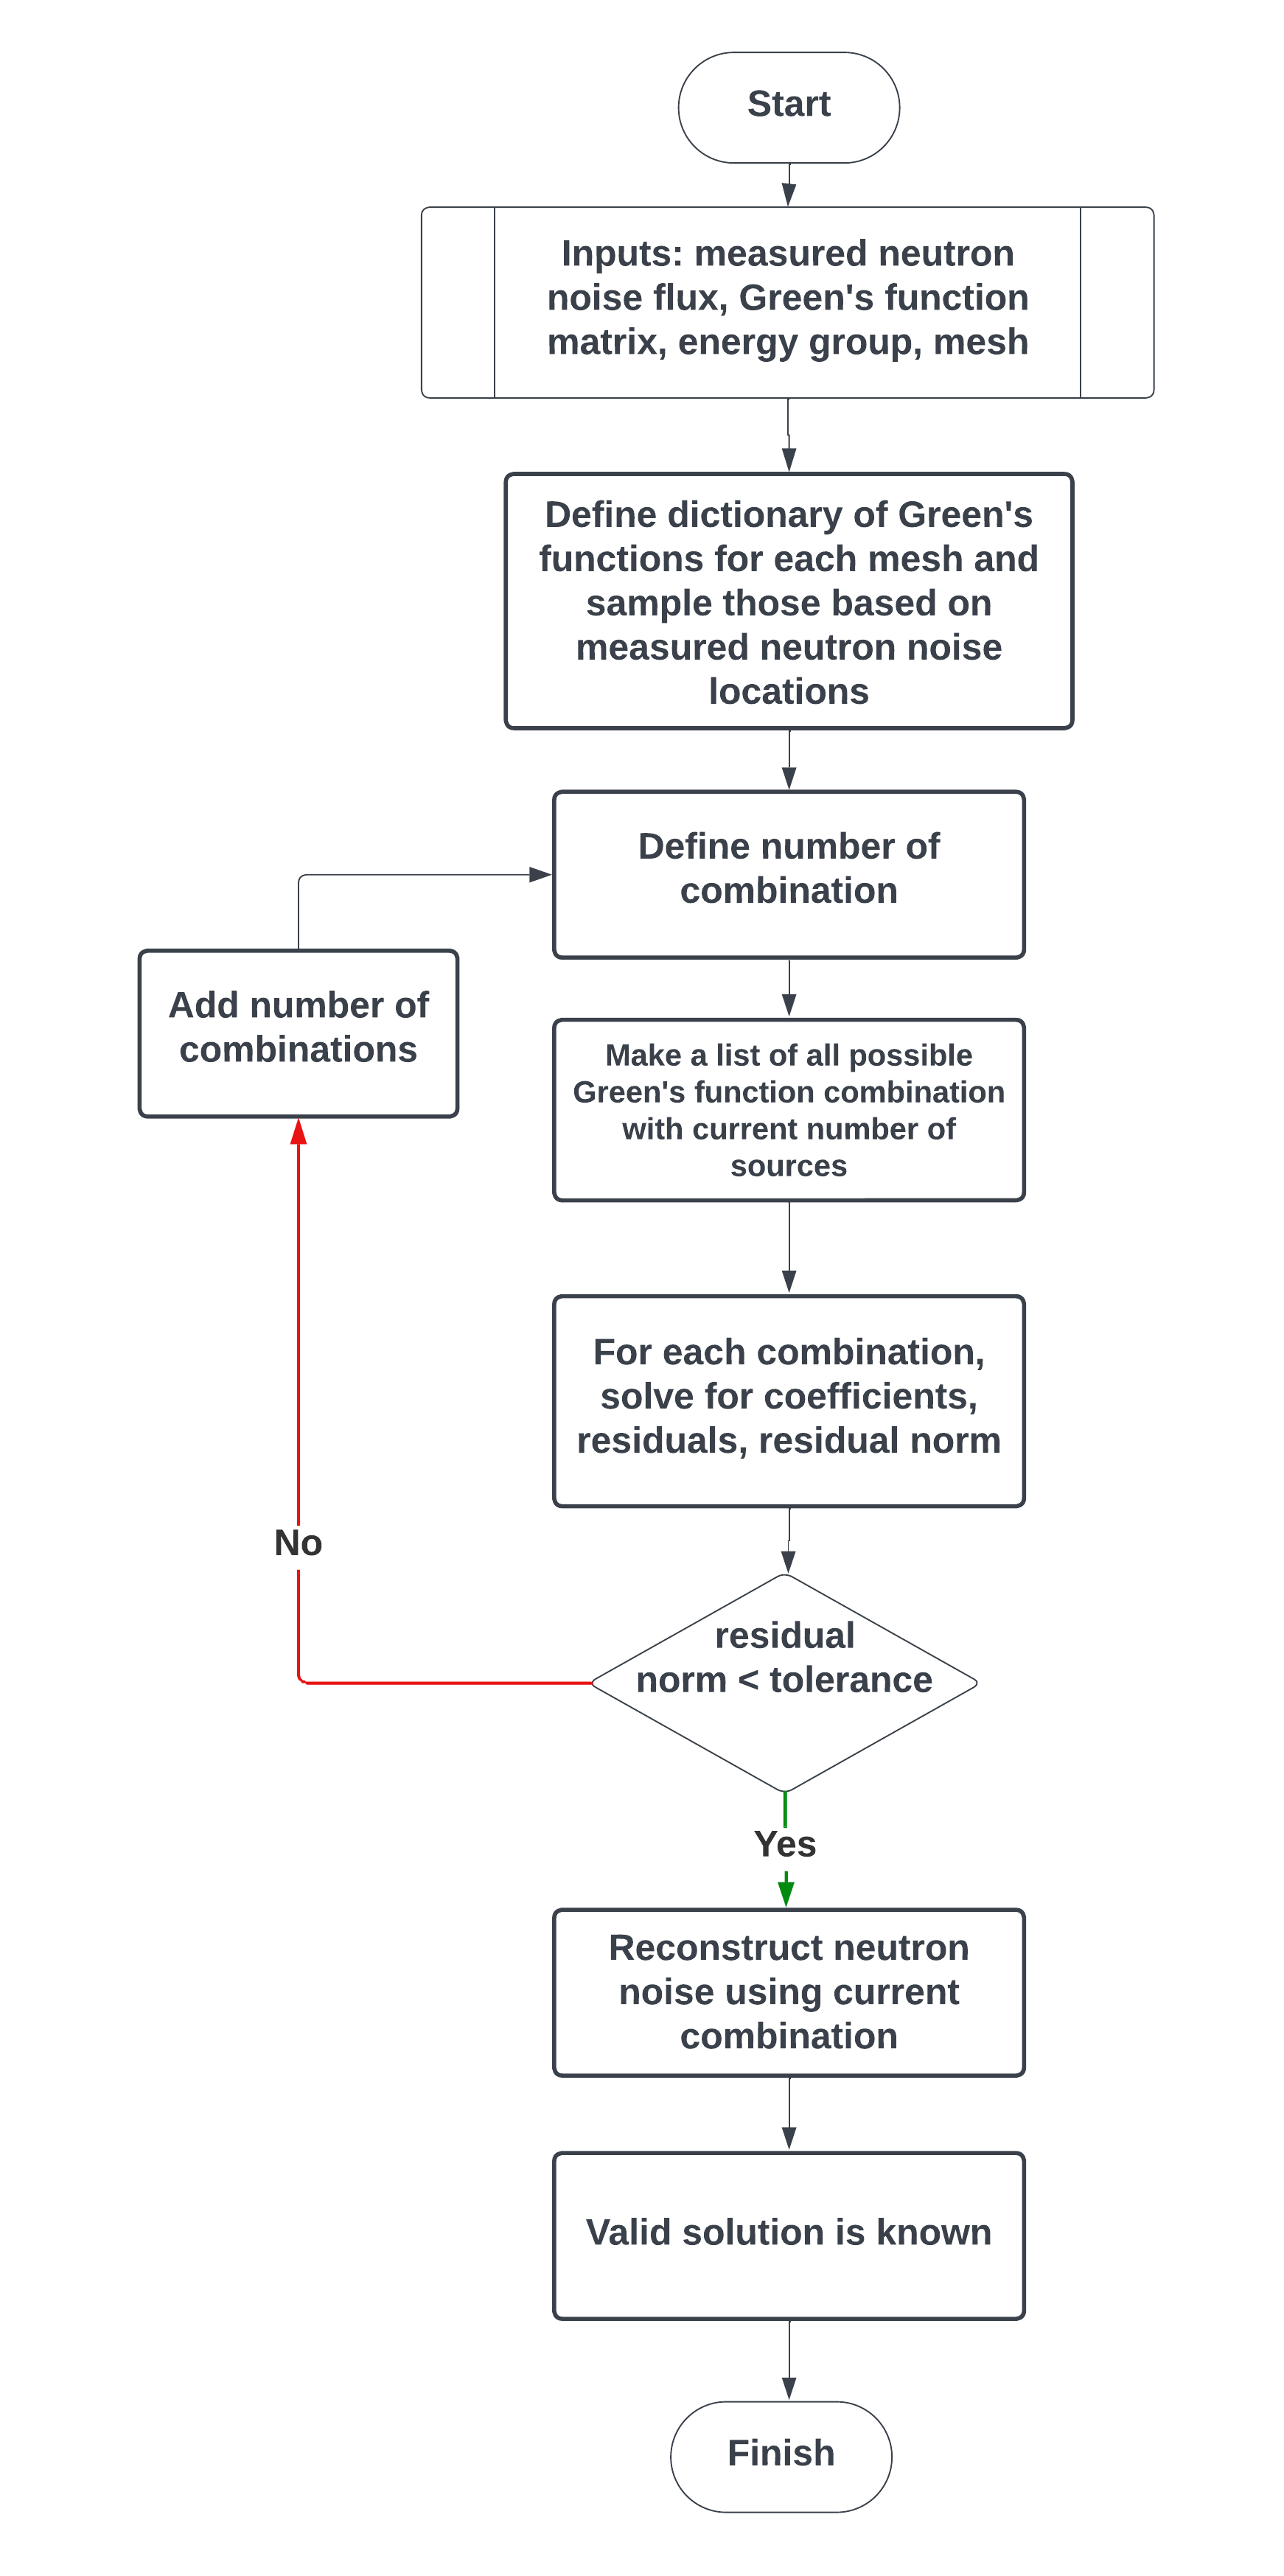
\includegraphics[width=0.6\textwidth]{figures/Brute Force Method.png}
        \caption{Flow diagram of brute force method}
        \label{fig:brute_force}
\end{figure}

The pseudo algorithm of the brute force method is described in Algorithm~\ref{alg:brute_force}.
\begin{algorithm}[H]
\caption{: Brute Force Method}
\label{alg:brute_force}
\begin{algorithmic}[1]
\Require Measured neutron noise $\delta \phi(\textbf{r}_{\text{meas}}, \omega)$, Green’s function matrix $G(\textbf{r}, \textbf{r}_p,\omega)$, energy groups $g$, mesh $N$
\Ensure reconstructed neutron noise $\delta \phi_{\text{BRUTE}}(\textbf{r}, \omega)$, unfolded source $S_{\text{BRUTE}}(\textbf{r}, \omega)$
\For{each group $g$} \Comment{\textbf{Construct Green’s function dictionary}}
    \For{each node $n$}
        \State Store columns of $G(\textbf{r}, \textbf{r}_p,\omega)$ in dictionary
    \EndFor
\EndFor
\State Sample columns only at measured (non-zero) indices

\For{$k = 1$ to total number of atoms} \Comment{\textbf{Brute-force search over subsets of atoms}}
    \State Calculate of subset of atoms of size $k$
    \ForAll{subsets of size $k$}
        \State Form matrix $A$ from selected atoms
        \State Solve least squares: $\mathbf{c} = \arg\min || \delta \phi(\textbf{r}_{\text{meas}}, \omega) - A \mathbf{c}||$
        \State Compute residual $r = ||\delta \phi(\textbf{r}_{\text{meas}}, \omega) - A \mathbf{c}||$
        \If{$r < \text{tolerance}$}
            \State Store valid $G_{g,n}$ solution
            \State Break all loops
        \EndIf
    \EndFor
\EndFor

\If{no valid solution is found, }
    \State \Return failure
\EndIf
\State Compute reconstructed neutron noise $\delta \phi_\text{BRUTE}(\textbf{r}, \omega) = \sum c_i G_{g_i,n_i}$ \Comment{\textbf{Reconstruct solution}}
\State Solve $S_{\text{BRUTE}}(\textbf{r}, \omega) = G^{-1}(\textbf{r}, \textbf{r}_p,\omega) \delta \phi_\text{BRUTE}(\textbf{r}, \omega)$
\State \textbf{Postprocess:} $S_{\text{BRUTE}}(\textbf{r}, \omega)$ file, $\delta \phi_\text{BRUTE}(\textbf{r}, \omega)$ file, plots. 
\end{algorithmic}
\end{algorithm}

This method is applied to unfold neutron noise sources for 2D and 3D HTTR geometries, which will be presented in Section \ref{sec:unfolding_application}.

\subsection{Greedy Method}

To put into perspective, the system of equations in Eq. \ref{eq:greens_function2} is an underconstrained system of linear equations, considering that the neutron noise is only known at the detectors’ positions. Methods from other fields have been used to solve such system of equations. One of the fields that has a similar problem is compressed sensing \cite{donohoCompressedSensing2006}. 

In compressed sensing, the system of linear equations is constructed based on the summation of a weighted set of basis functions. These sets of basis functions are then used to match the set of measurements  \cite{priceSimplifiedMatchingPursuits2024}. In compressed sensing, the solution of the underconstrained equation is a set of basis functions that minimizes the L0-norm of the solution vector. In reactor physics, this method has been applied in various contexts, including neutron flux distribution \cite{bahugunaSignalRecoverySparse2017, bahugunaCompressedSensingArtificial2018}, temperature distribution construction \cite{priceSimplifiedMatchingPursuits2024}, and reduced-order modeling \cite{gongDataEnabledPhysicsInformedMachine2022}.

For the application of neutron noise reconstruction, a method inspired by greedy algorithms, such as matching pursuit \cite{mallatMatchingPursuitsTimefrequency1993}, is employed. This is because the sparsity of the linear system is explicitly enforced with the L0-norm \cite{priceSimplifiedMatchingPursuits2024}. In a matching pursuit, the basis function used for the construction is orthonormal \cite{mallatMatchingPursuitsTimefrequency1993}. Meanwhile, the basis function in this case is the Green's function, which is not orthonormal. Therefore, a different approach is needed to utilize the Green's function as the basis function. The goal of the greedy method is to find the polynomial combination of Green's function to solve Eq. \ref{eq:greens_function2}. This can be written as:
\begin{equation}
    \min \| G(\textbf{r},\omega) \|_0 \quad \text{subject to} \quad \delta \phi = G(\textbf{r}) S 
\end{equation}

The general idea of the greedy method is to pick a mesh represented by the Green's function ($G(\textbf{r},\omega)$) in every iteration until it reaches the desired residual norm. There are two iterations in the greedy method, the inner and outer iterations. The outer iteration starts with choosing a mesh as the initial guess of the solution. From the mesh, we can extract the Green's function corresponding to the mesh. Then, it continues to the inner iteration. It starts with a single mesh $i$, where we define the initial residual norm:
\begin{equation}
    r_i^0 =  \| \delta \phi \|_2
\end{equation}
At each step of the inner iteration, all meshes $j \neq i$ are examined. Each candidate mesh $j$ is temporarily appended to the current selection $j^*$ (which initially contains mesh $i$), and the Green's function corresponding the mesh is extracted. Then, the coefficients $S$ for this selection are calculated using the Least Square method. After the coefficients are calculated, the residual norm for this selection is computed. The selection $j^*$ that yields the smallest residual norm is then selected as the next mesh to include. This selection can be expressed as,
\begin{equation}
    \varepsilon(j) = \min_{G_j} \| G(j, \mathbf{r}, \omega) S - r_i^0 \|_2
\end{equation}
The selected mesh $j^*$ is then carried over to the next inner iteration. The inner iteration is performed until the desired residual norm is reached. The residual norm tolerance was set to $10^{-10}$, which corresponds to the residual norm of the solution brute force. It is then saved in a list of valid solutions. After that, the outer iterations continue to pick different mesh as a starting point for the inner iteration. The output of the outer iteration is a list of valid solutions with length  $(\text{group} \times N)$. From these valid solutions, the solution that has the least number of mesh combination is selected as the correct solution for the neutron noise.

The flow diagram of the method is described in Figure \ref{fig:greedy_method}.
\begin{figure}[H]
        \centering
        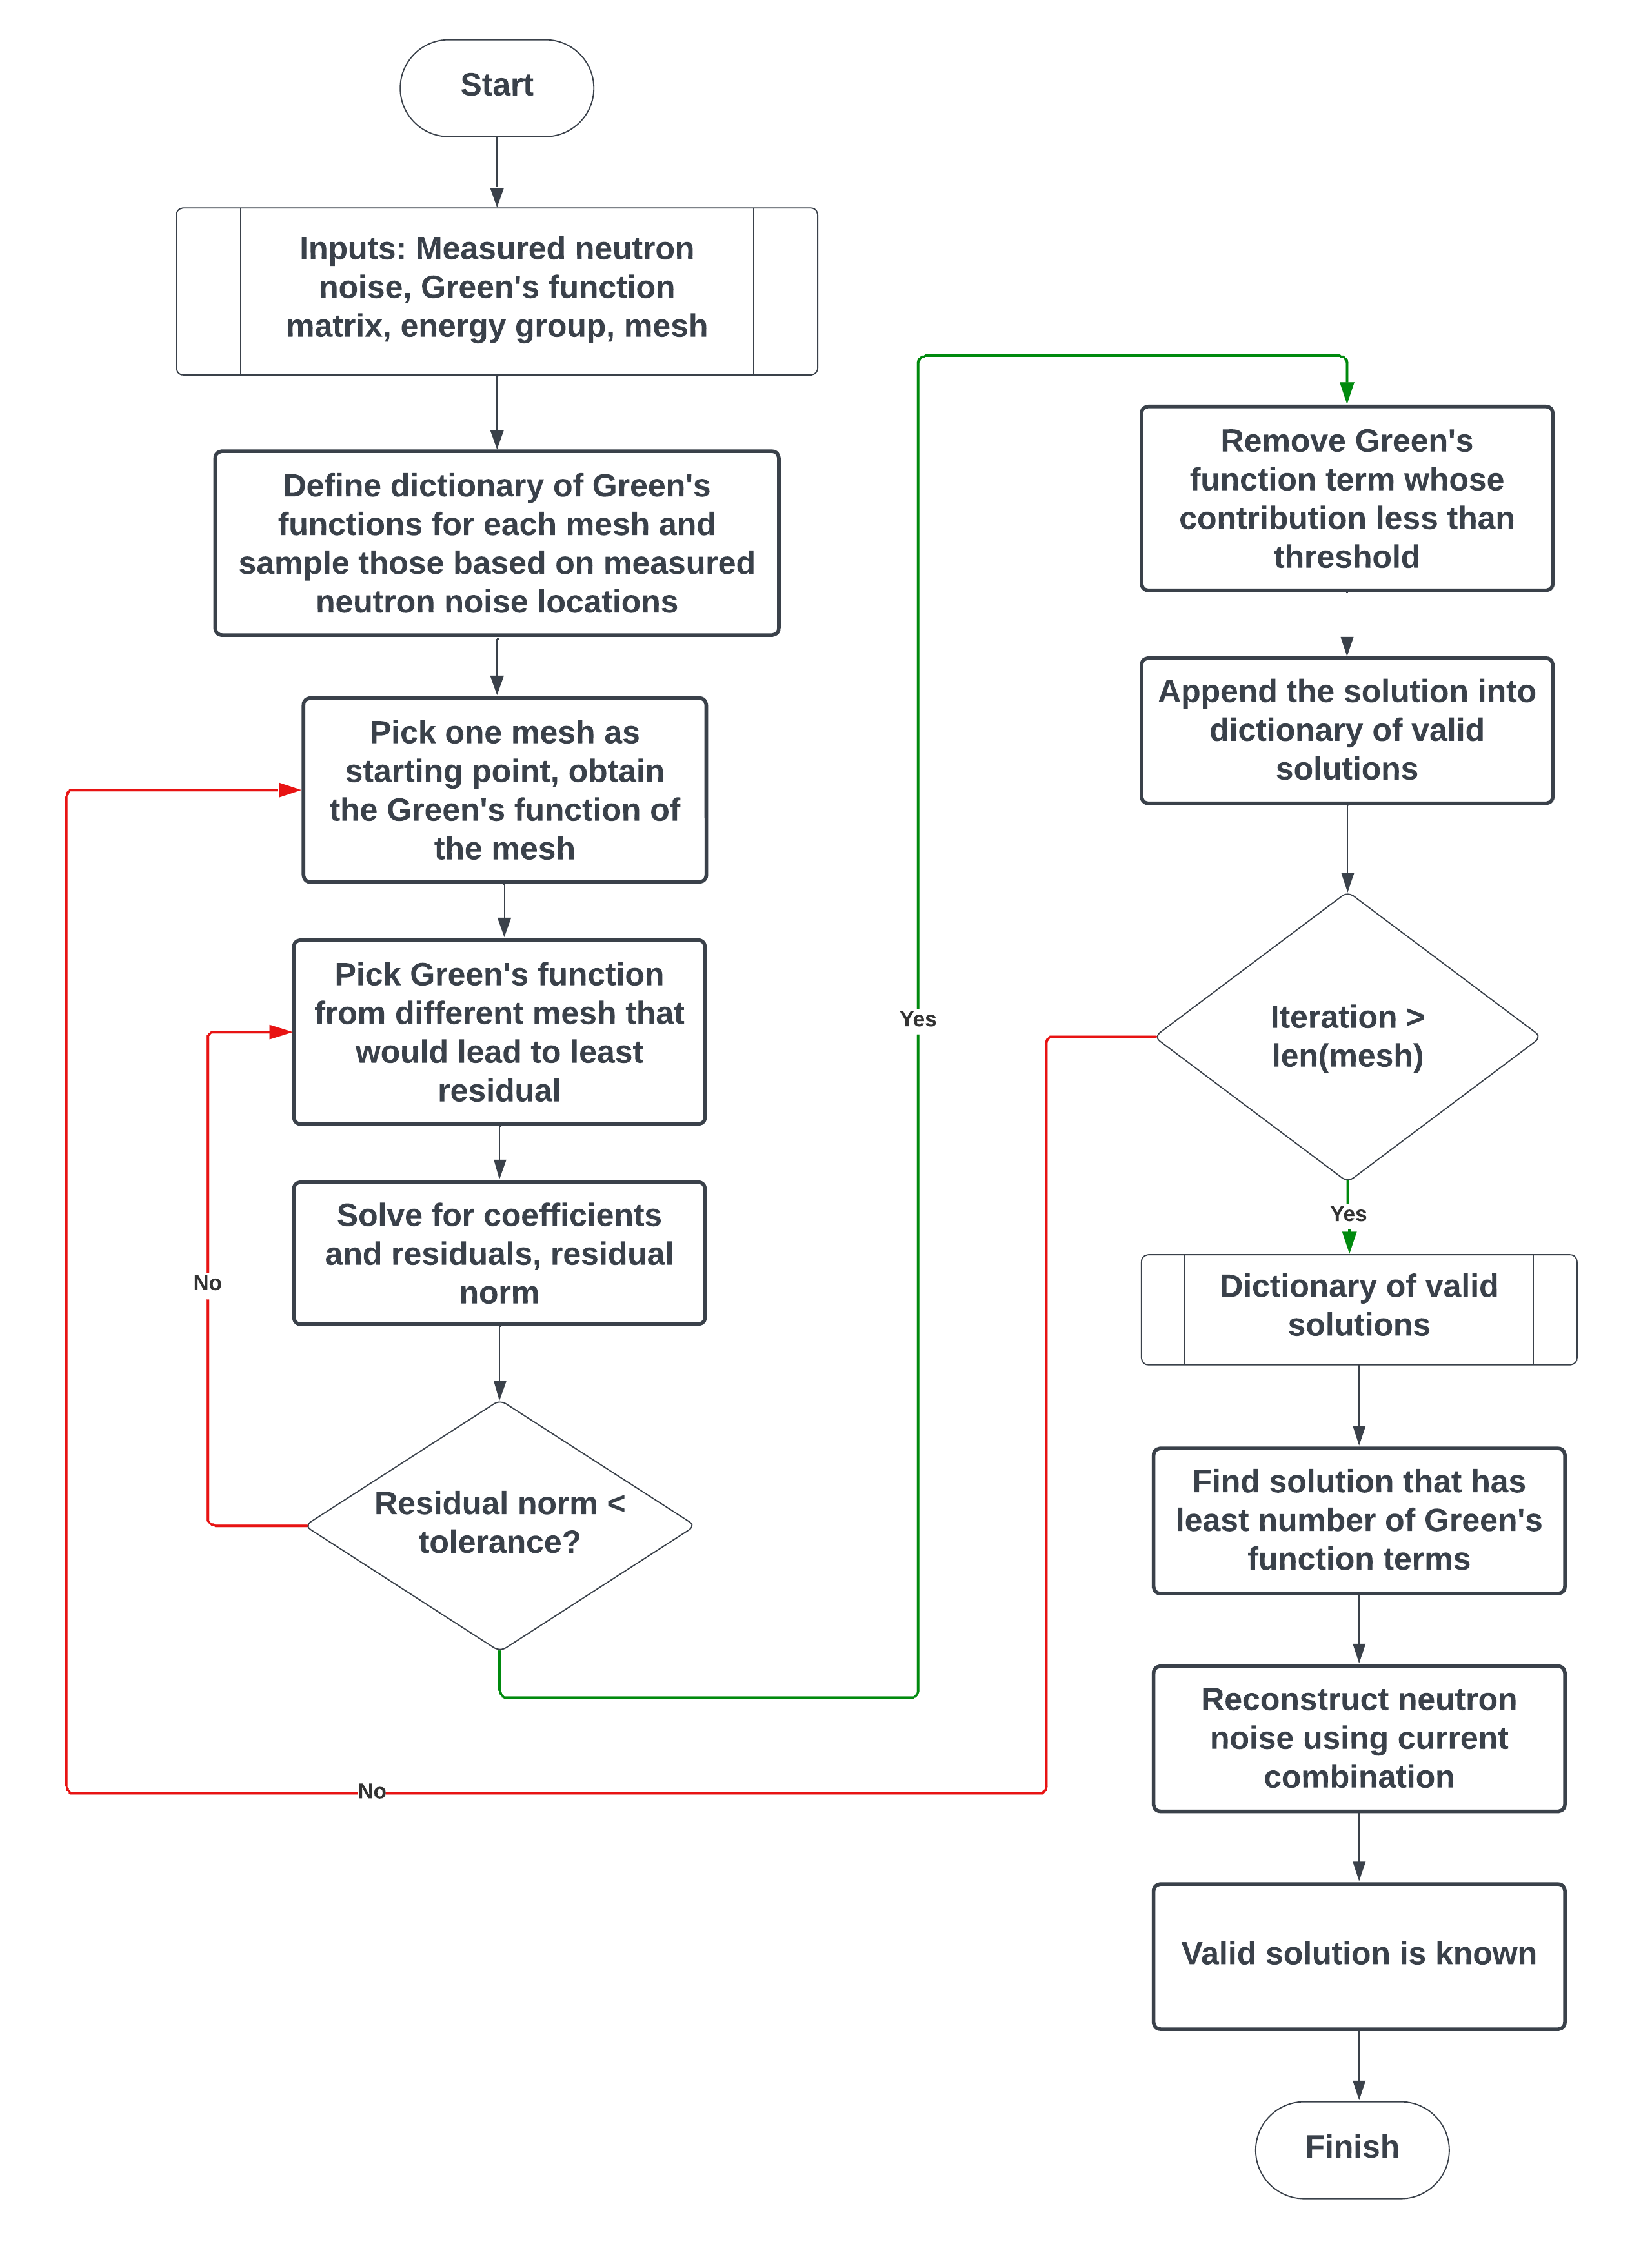
\includegraphics[width=0.6\textwidth]{figures/Greedy Method.png}
        \caption{Flow diagram of greedy method}
        \label{fig:greedy_method}
\end{figure}

The pseudo algorithm of the greedy method  is described in Algorithm~\ref{alg:greedy_unfold}.
\begin{algorithm}[H]
\caption{: Greedy Method}
\label{alg:greedy_unfold}
\begin{algorithmic}[1]
\Require Measured neutron noise $\delta \phi(\textbf{r}_{\text{meas}}, \omega)$, Green’s function matrix $G(\textbf{r}, \textbf{r}_p,\omega)$, energy groups $g$, mesh $N$
\Ensure reconstructed neutron noise $\delta \phi_{\text{GREEDY}}(\textbf{r}, \omega)$, unfolded source $S_{\text{GREEDY}}(\textbf{r}, \omega)$
\For{each group $g$} \Comment{\textbf{Construct Green’s function dictionary}}
    \For{each node $n$}
        \State Store columns of $G(\textbf{r}, \textbf{r}_p,\omega)$ in a dictionary
    \EndFor
\EndFor
\State Sample columns only at measured (non-zero) indices
\State Initialize solution sets: valid solutions $\gets \{\}$
\For{each candidate column $i$ in the dictionary subset} \Comment{\textbf{Greedy column selection}}
    \State Initialize residual $r \gets \delta \phi(\textbf{r}_{\text{meas}}, \omega)$
    \State Initialize selected column set $j^* \gets \{i\}$
    \While{$||\text{residual}||_2 > \text{tol}$}
        \State For each column $j \neq j*$, temporarily appended to the current selection $j^*$
        \State Compute the residual norm of the least squares fit with $S \cup \{j\}$
        \State Select column $j^*$ that minimizes residual norm
        \State Update $S \gets S \cup \{j^*\}$
        \State Update residual
    \EndWhile
    \State Recompute least-squares coefficients $\mathbf{c}$ of selected atom set $j^*$
    \State Remove columns with negligible contributions ($|c_i|/\max |c| < \tau$)    
    \State Store selected set $j^* \rightarrow$ valid solutions
\EndFor
\If{valid solutions exist} \Comment{\textbf{Select best solution}}
    \State Choose solution with minimal column count
    \State Compute reconstructed neutron noise: $\delta \phi_{\text{GREEDY}}(\textbf{r}, \omega) = \sum c_i G_i$
\Else
    \State \Return failure
\EndIf
\State Solve $S_{\text{GREEDY}}(\textbf{r}, \omega) = G^{-1}(\textbf{r}, \textbf{r}_p,\omega) \delta \phi_\text{GREEDY}(\textbf{r}, \omega)$
\State \textbf{Postprocess:} $S_{\text{GREEDY}}(\textbf{r}, \omega)$ file, $\delta \phi_\text{GREEDY}(\textbf{r}, \omega)$ file, plots. 
\end{algorithmic}
\end{algorithm}

This method is applied to unfold neutron noise sources for 2D and 3D HTTR geometries, which will be presented in Section \ref{sec:unfolding_application}.

\section{Application of HTTR Core}
\label{sec:unfolding_application}

In these cases, it is assumed that the detectors installed in the reactor can accurately measure neutron noise in both the fast and thermal energy groups. Any intrinsic detector noise is considered to have been removed, so the measured noise represents only the reactor-induced neutron noise. For the 2D HTTR case, there are 21 detectors that can accurately measure neutron noise. For the 3D HTTR case, there are also 21 detectors. Each detector can accurately detect neutron noise for the whole fuel column.

\subsection{2D HTTR with Absorber of Variable Strength Source}

\subsubsection{Single Noise Source}

In this simulation, a single mesh AVS source is unfolded using both the existing and novel methods. The simulation is done with a constant frequency of 1 Hz.  Figure \ref{fig:map_S_2DHTTR_AVS1S} shows the location of the AVS source.
\begin{figure}[H]
        \centering
        \begin{subfigure}{.48\textwidth}
          \centering
          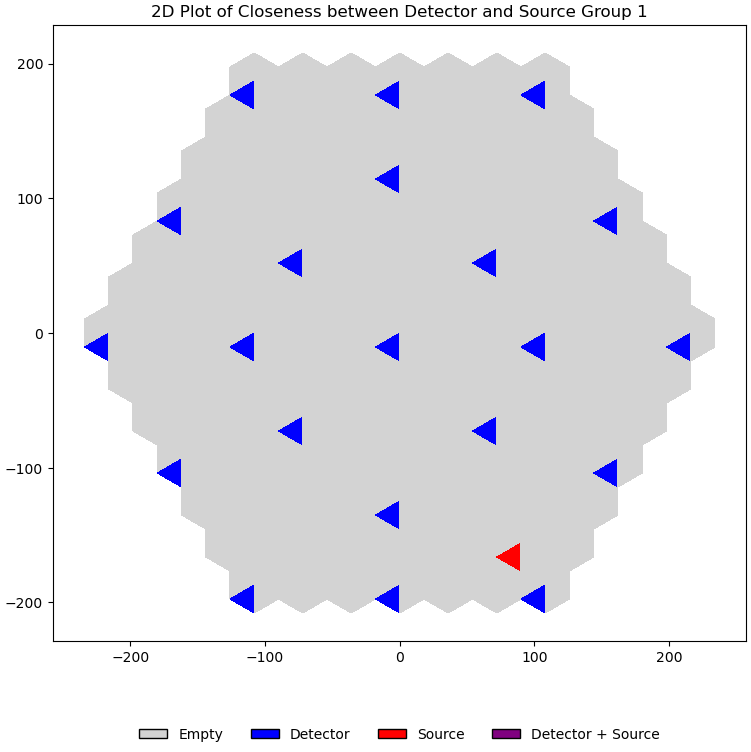
\includegraphics[width=\linewidth]{figures/OBJECTIVES6_TEST_SUITE_2DTriMG_HTTR_level1_iter2_closeness_det_S_categorical_G1.png}
        \end{subfigure}
        \hfill
        \begin{subfigure}{.48\textwidth}
          \centering
          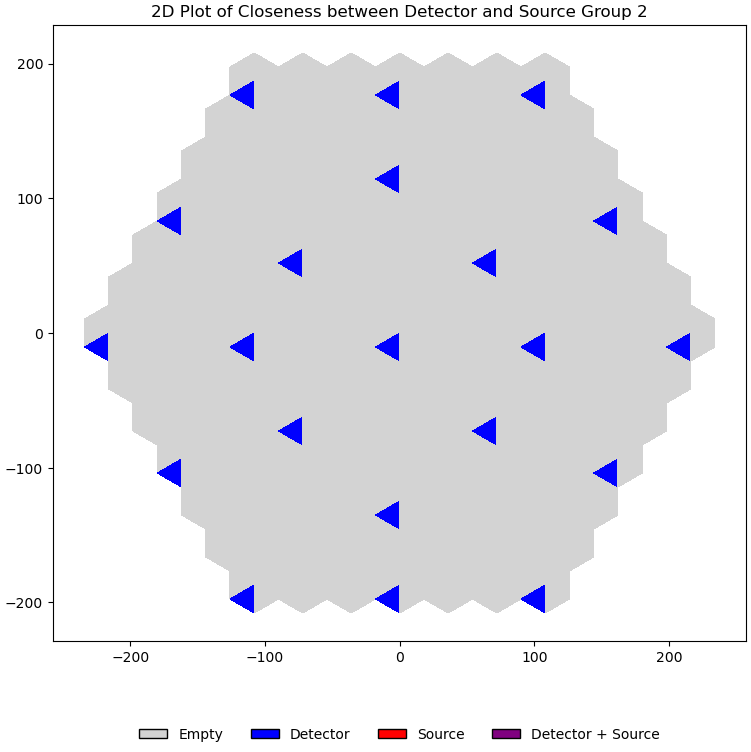
\includegraphics[width=\linewidth]{figures/OBJECTIVES6_TEST_SUITE_2DTriMG_HTTR_level1_iter2_closeness_det_S_categorical_G2.png}
        \end{subfigure}
        \caption{Location of source and detectors in the 2D HTTR case}
        \label{fig:map_S_2DHTTR_AVS1S}
\end{figure}

The results of the simulations are described in Table \ref{table:unfold_2DHTTR_AVS1S}.
\begin{table}[H]
        \centering
        \caption{Single noise source in 2D HTTR}
        \label{table:unfold_2DHTTR_AVS1S}
        \begin{tabular}{ | M{2cm} | M{1.5cm} | M{1.5cm} | M{4.5cm} | M{1.5cm} | } 
         \hline
         \textbf{Method} & \textbf{Energy Group} & \textbf{Hex Number} & \textbf{Neutron Noise Source} ($n/cm^3$) & \textbf{Match?}  \\
         \hline
         Reference & 1 & 14 & $-4.893 \times 10^{-5}+0.000i$ & --  \\
         \hline
         Inversion & 1 & 1 & $0.000+0.000i$ & No  \\
         \hline
         Zoning & 2 & 89 & $-5.635 \times 10^{-6}+4.056 \times 10^{-6}i$ & No  \\
         \hline
         Scanning & 1 & 14 & $-4.893 \times 10^{-5}+0.000i$ & Yes  \\
         \hline
         Brute Force & 1 & 14 & $-4.893 \times 10^{-5}+0.000i$ & Yes  \\
         \hline
         Greedy & 1 & 14 & $-4.893 \times 10^{-5}+0.000i$ & Yes  \\
         \hline
        \end{tabular}
\end{table}
The results show that the inversion and zoning method fails to unfold the neutron noise source. For the inversion method, this is due to the sparsity of the measured neutron noise, which results in poor interpolation quality. For the zoning method, it successfully identifies a location, but it is not the correct location of the neutron noise source. This is due to the limitation of the zoning method, where the number of fuel assemblies in each zone must be arranged in a specific way to match the number of detectors. On the other hand, scanning, brute force, and greedy methods manage to unfold the neutron noise source. This is an expected behavior. For the scanning method, it works well for a single mesh source, since it minimizes the difference between the neutron noise ratio and Green’s function ratio (See Eq. \ref{eq:scan_min}). The minimum difference is in the noise source location. For the brute force and greedy method, the method works well and matches the reference solution.

\subsubsection{Two Noise Sources}

In this simulation, a two-mesh AVS source is unfolded using both the existing and novel methods. The simulation is done with a constant frequency of 0.056 Hz. Figure \ref{fig:map_S_2DHTTR_AVS2S} shows the location of the AVS source.
\begin{figure}[H]
        \centering
        \begin{subfigure}{.48\textwidth}
          \centering
          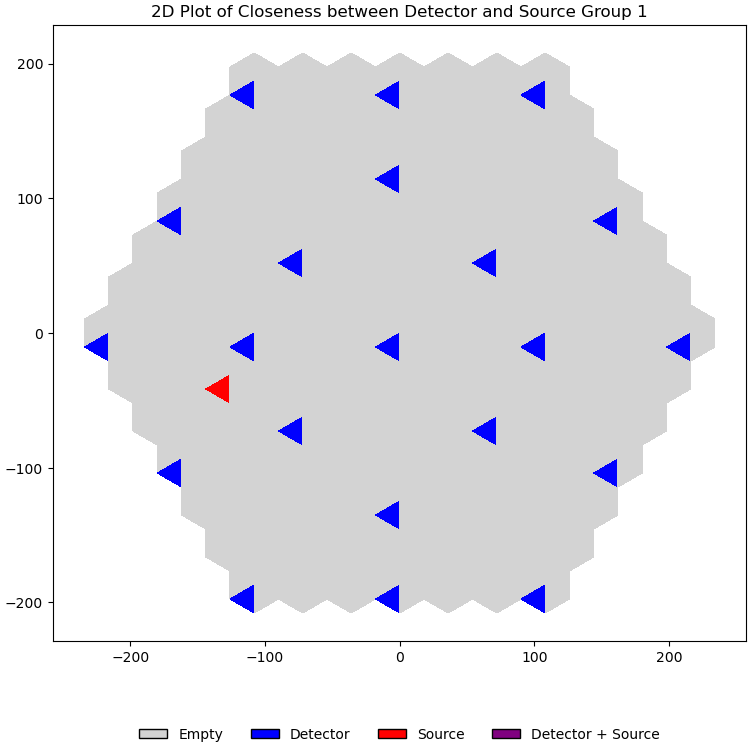
\includegraphics[width=\linewidth]{figures/OBJECTIVES6_TEST_SUITE_2DTriMG_HTTR_level1_iter18_closeness_det_S_categorical_G1.png}
        \end{subfigure}
        \hfill
        \begin{subfigure}{.48\textwidth}
          \centering
          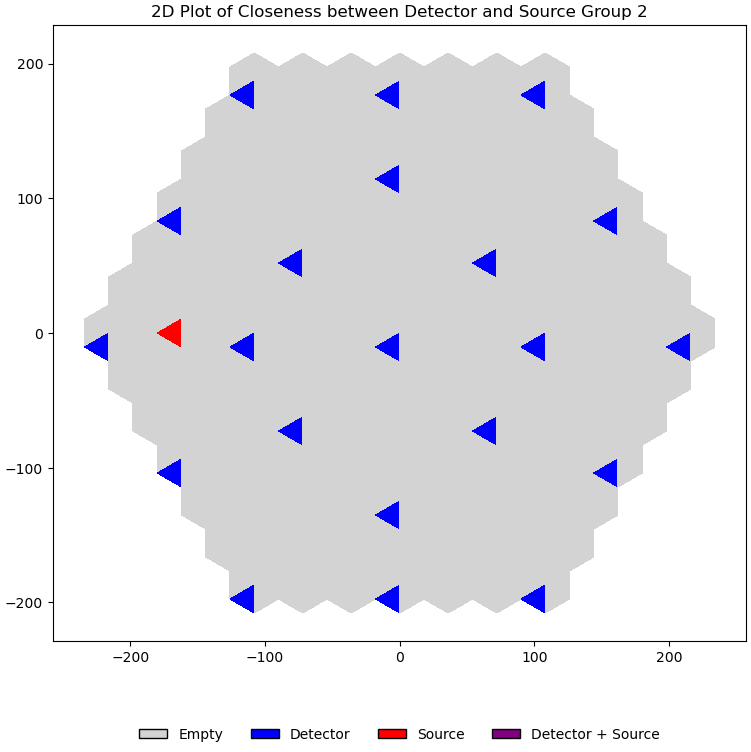
\includegraphics[width=\linewidth]{figures/OBJECTIVES6_TEST_SUITE_2DTriMG_HTTR_level1_iter18_closeness_det_S_categorical_G2.png}
        \end{subfigure}
        \caption{Location of sources and detectors in the 2D HTTR case}
        \label{fig:map_S_2DHTTR_AVS2S}
\end{figure}

The results of the simulations are described in Table \ref{table:unfold_2DHTTR_AVS2S}.
\begin{table}[H]
        \centering
        \caption{Two noise sources in 2D HTTR}
        \label{table:unfold_2DHTTR_AVS2S}
        \begin{tabular}{ | M{2cm} | M{1.5cm} | M{1.5cm} | M{4.5cm} | M{1.5cm} | } 
         \hline
         \textbf{Method} & \textbf{Energy Group} & \textbf{Hex Number} & \textbf{Neutron Noise Source} ($
         n/cm^3$) & \textbf{Match?}  \\
         \hline
         \multirow{2}{*}{Reference} & 1 & 48 & $-1.882 \times 10^{-3}+0.000i$ & --  \\
         \cline{2-5}                & 2 & 60 & $-5.189 \times 10^{-3}-4.670 \times 10^{-3}i$ & --  \\
         \hline
         \multirow{2}{*}{Inversion} & 1 & 1 & $0.000+0.000i$ & No  \\
         \cline{2-5}                & 1 & 2 & $0.000+0.000i$ & No  \\
         \hline
         \multirow{2}{*}{Zoning} & 1 & 86 & $-2.383 \times 10^{-3}+6.761 \times 10^{-4}i$ & No  \\
         \cline{2-5}             & 1 & 89 & $-2.201 \times 10^{-3}+9.212 \times 10^{-4}i$ & No  \\
         \hline
         \multirow{2}{*}{Scanning} & 2 & 60 & $-1.033 \times 10^{-2}-4.138 \times 10^{-3}i$ & No  \\
         \cline{2-5}               & 1 & 1 & $0.000+0.000i$ & No  \\
         \hline
         \multirow{2}{*}{Brute Force} & 1 & 48 & $-1.882 \times 10^{-3}+0.000i$ & Yes  \\
         \cline{2-5}                  & 2 & 60 & $-5.189 \times 10^{-3}-4.670 \times 10^{-3}i$ & Yes  \\
         \hline
         \multirow{2}{*}{Greedy} & 1 & 48 & $-1.882 \times 10^{-3}+0.000i$ & Yes  \\
         \cline{2-5}             & 2 & 60 & $-5.189 \times 10^{-3}-4.670 \times 10^{-3}i$ & Yes  \\
         \hline
        \end{tabular}
\end{table}
The results show that the inversion, zoning, and scanning method fails to unfold the neutron noise source. The inversion and zoning method is expected to fail, since it fails in a single source. The scanning method fails due to the method’s limitation, as it only points to one location that minimizes the ratio difference in Eq. \ref{eq:scan_min}. On the other hand, brute force and greedy methods manage to unfold the neutron noise source. This is expected behavior for both methods.

\subsubsection{Three Noise Sources}

In this simulation, a three-mesh AVS source is unfolded using both the existing and novel methods. The simulation is done with a constant frequency of 1 Hz. Figure \ref{fig:map_S_2DHTTR_AVS3S} shows the location of the AVS source.
\begin{figure}[H]
        \centering
        \begin{subfigure}{.48\textwidth}
          \centering
          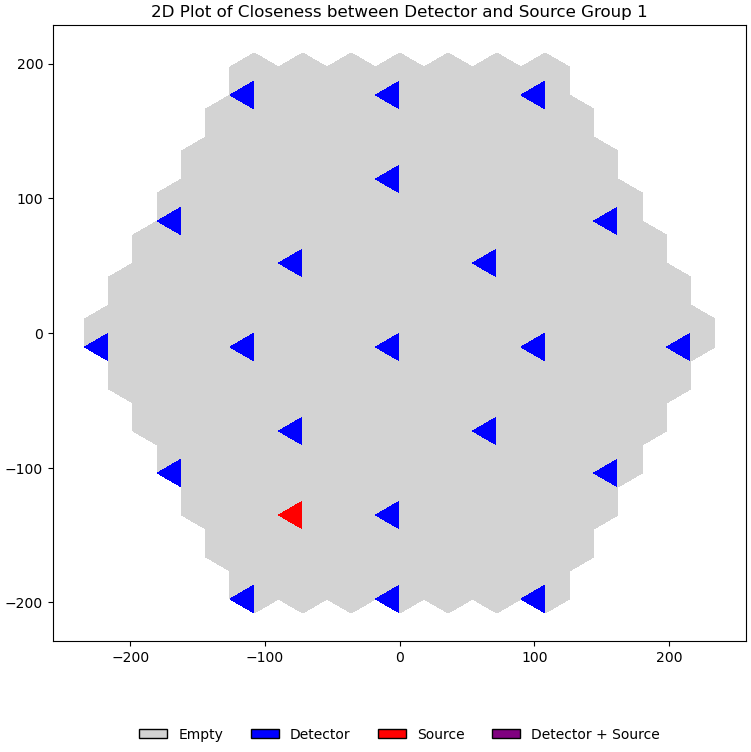
\includegraphics[width=\linewidth]{figures/OBJECTIVES45_TEST10_2DTriMG_HTTR_AVS3S_level1_closeness_det_S_categorical_G1.png}
        \end{subfigure}
        \hfill
        \begin{subfigure}{.48\textwidth}
          \centering
          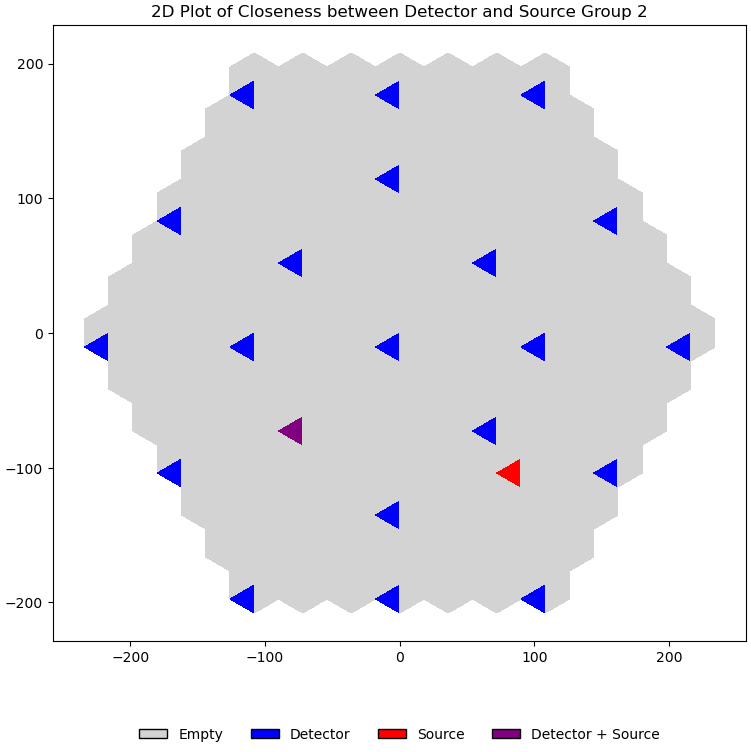
\includegraphics[width=\linewidth]{figures/OBJECTIVES45_TEST10_2DTriMG_HTTR_AVS3S_level1_closeness_det_S_categorical_G2.png}
        \end{subfigure}
        \caption{Location of sources and detectors in the 2D HTTR case}
        \label{fig:map_S_2DHTTR_AVS3S}
\end{figure}

The results of the simulations are described in Table \ref{table:unfold_2DHTTR_AVS3S}.
\begin{table}[H]
        \centering
        \caption{Three noise sources in 2D HTTR}
        \label{table:unfold_2DHTTR_AVS3S}
        \begin{tabular}{ | M{2cm} | M{1.5cm} | M{1.5cm} | M{4.5cm} | M{1.5cm} | } 
         \hline
         \textbf{Method} & \textbf{Energy Group} & \textbf{Hex Number} & \textbf{Neutron Noise Source} ($n/cm^3$) & \textbf{Match?}  \\
         \hline
         \multirow{3}{*}{Reference} & 1 & 18 & $-2.795 \times 10^{-8}+0.000i$ & --  \\
         \cline{2-5}                & 2 & 32 & $-3.342 \times 10^{-6}+0.000i$ & --  \\
         \cline{2-5}                & 2 & 38 & $-1.053 \times 10^{-4}+0.000i$ & --  \\
         \hline
         \multirow{3}{*}{Inversion} & 1 & 1 & $0.000+0.000i$ & No  \\
         \cline{2-5}                & 1 & 45 & $0.000+0.000i$ & No  \\
         \cline{2-5}                & 2 & 61 & $0.000+0.000i$ & No  \\
         \hline
         \multirow{3}{*}{Zoning} & 2 & 39 & $-1.915 \times 10^{-4}+9.311 \times 10^{-5}i$ & No \\
         \cline{2-5}             & 2 & 39 & $-1.753 \times 10^{-4}+9.751 \times 10^{-5}i$ & No \\
         \cline{2-5}             & 2 & 39 & $-1.648 \times 10^{-4}+8.764 \times 10^{-5}i$ & No \\
         \hline
         \multirow{3}{*}{Scanning} & 2 & 37 & $-1.062 \times 10^{-4}+1.096 \times 10^{-7}i$ & No  \\
         \cline{2-5}               & 1 & 1 & $0.000+0.000i$ & No  \\
         \cline{2-5}               & 1 & 2 & $0.000+0.000i$ & No  \\
         \hline
         \multirow{3}{*}{Brute Force} & 1 & 18 & $-2.795 \times 10^{-8}+0.000i$ & Yes  \\
         \cline{2-5}                  & 2 & 32 & $-3.342 \times 10^{-6}+0.000i$ & Yes  \\
         \cline{2-5}                  & 2 & 38 & $-1.053 \times 10^{-4}+0.000i$ & Yes  \\
         \hline
         \multirow{3}{*}{Greedy} & 1 & 18 & $-2.795 \times 10^{-8}+0.000i$ & Yes  \\
         \cline{2-5}             & 2 & 32 & $-3.342 \times 10^{-6}+0.000i$ & Yes  \\
         \cline{2-5}             & 2 & 38 & $-1.053 \times 10^{-4}+0.000i$ & Yes  \\
         \hline
        \end{tabular}
\end{table}
Similar to the two noise source problem, the results show that the inversion, zoning, and scanning method fails to unfold the neutron noise source. On the other hand, brute force and greedy methods manage to unfold the neutron noise source. This is expected behavior for both methods.

\subsection{3D HTTR with Absorber of Variable Strength Source}

\subsubsection{Single Noise Source}

In this simulation, a single mesh AVS source is unfolded using both the existing and novel methods. The simulation is done with a constant frequency of 1 Hz. The noise source is located at $Z=5$, thermal energy group. Figure \ref{fig:map_S_3DHTTR_AVS1S} shows the location of the AVS source.
\begin{figure}[H]
        \centering
        \begin{subfigure}{.48\textwidth}
          \centering
          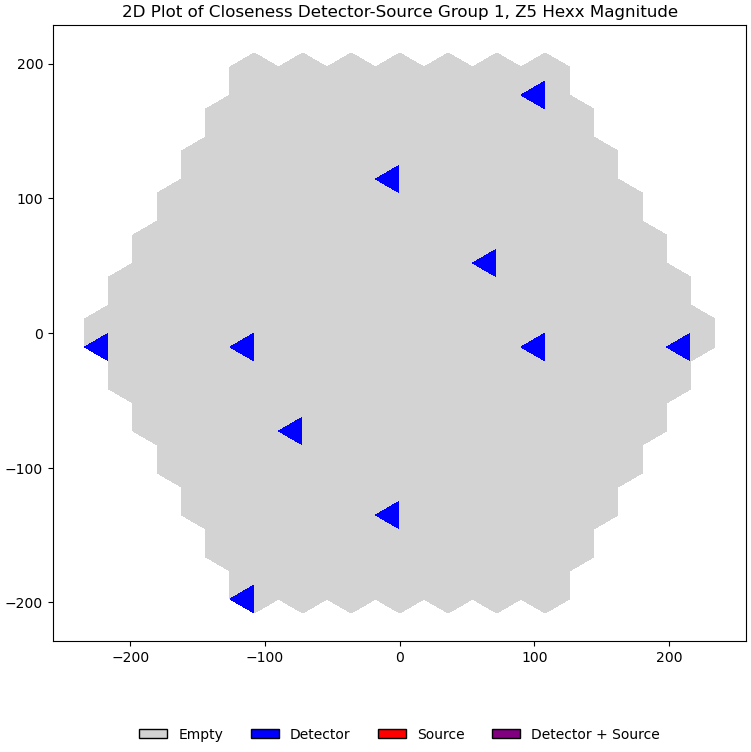
\includegraphics[width=\linewidth]{figures/OBJECTIVES45_TEST07_3DTriMG_HTTR_AVS_level1_closeness_det_S_categorical_G1_Z5.png}
        \end{subfigure}
        \hfill
        \begin{subfigure}{.48\textwidth}
          \centering
          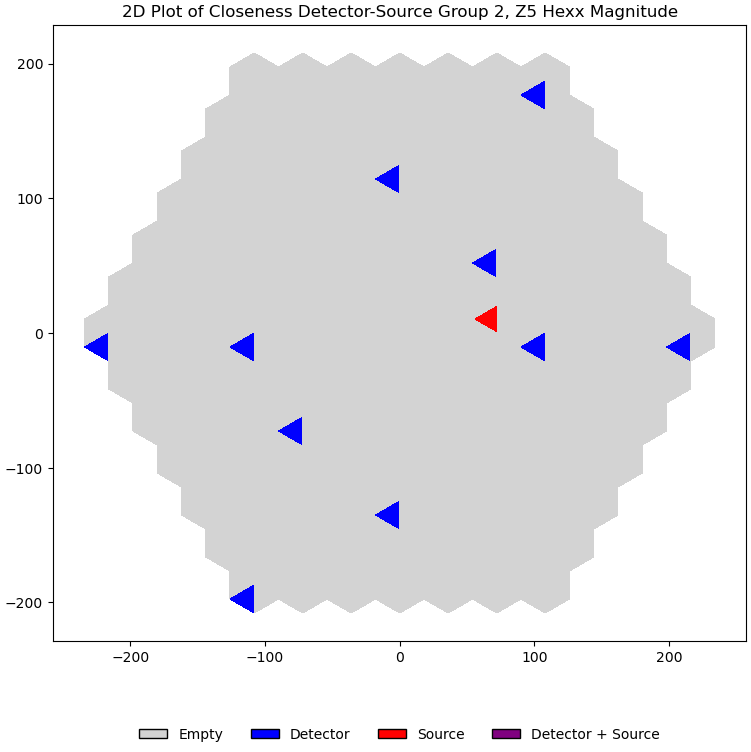
\includegraphics[width=\linewidth]{figures/OBJECTIVES45_TEST07_3DTriMG_HTTR_AVS_level1_closeness_det_S_categorical_G2_Z5.png}
        \end{subfigure}
        \caption{Location of source and detectors in the 3D HTTR single source case}
        \label{fig:map_S_3DHTTR_AVS1S}
\end{figure}

The results of the simulations are described in Table \ref{table:unfold_3DHTTR_AVS1S}.
\begin{table}[H]
        \centering
        \caption{Single noise source in 3D HTTR}
        \label{table:unfold_3DHTTR_AVS1S}
        \begin{tabular}{ | M{2cm} | M{1.5cm} | M{1.5cm} | M{1.5cm} | M{4cm} | M{1.5cm} | } 
         \hline
         \textbf{Method} & \textbf{Energy Group} & \textbf{Axial Level} & \textbf{Hex Number} & \textbf{Neutron Noise Source} ($n/cm^3$) & \textbf{Match?}  \\
         \hline
         Reference & 1 & 5 & 1 & $-4.912 \times 10^{-6} + 0.000i$ & -- \\
         \hline
         Inversion & 1 & 1 & 1 & $0.000 + 0.000i$ & No \\
         \hline
         Zoning & 2 & 3 & 9 & $-2.857 \times 10^{-6} + 0.000i$ & No \\
         \hline
         Scanning & 1 & 5 & 1 & $-4.912 \times 10^{-6} + 0.000i$ & Yes \\
         \hline
         Brute Force & 1 & 5 & 1 & $-4.912 \times 10^{-6} + 0.000i$ & Yes \\
         \hline
         Greedy & 1 & 5 & 1 & $-4.912 \times 10^{-6} + 0.000i$ & Yes \\
         \hline
        \end{tabular}
\end{table}
Similar to the results of a single mesh in the 2D HTTR case, the results show that the inversion and zoning method fails to unfold the neutron noise source. The scanning, brute force, and greedy methods manage to unfold the neutron noise source correctly. This is  expected behavior for the methods.

\subsubsection{Two Noise Source}

In this simulation, a two-mesh AVS source is unfolded using both the existing and novel methods. The simulation is done with a constant frequency of 1 Hz. There are 21 detectors in this case. Each detector can accurately detect neutron noise for the whole fuel column. The noise source is located in two different groups and axial levels. One source is located at $Z=4$ (near midplane) and fast group, while the other source is located at $Z=9$ (bottom of the core) and thermal group. Figure \ref{fig:map_S_3DHTTR_AVS2S} shows the location of the AVS source.
\begin{figure}[H]
        \centering
        \begin{subfigure}{.48\textwidth}
          \centering
          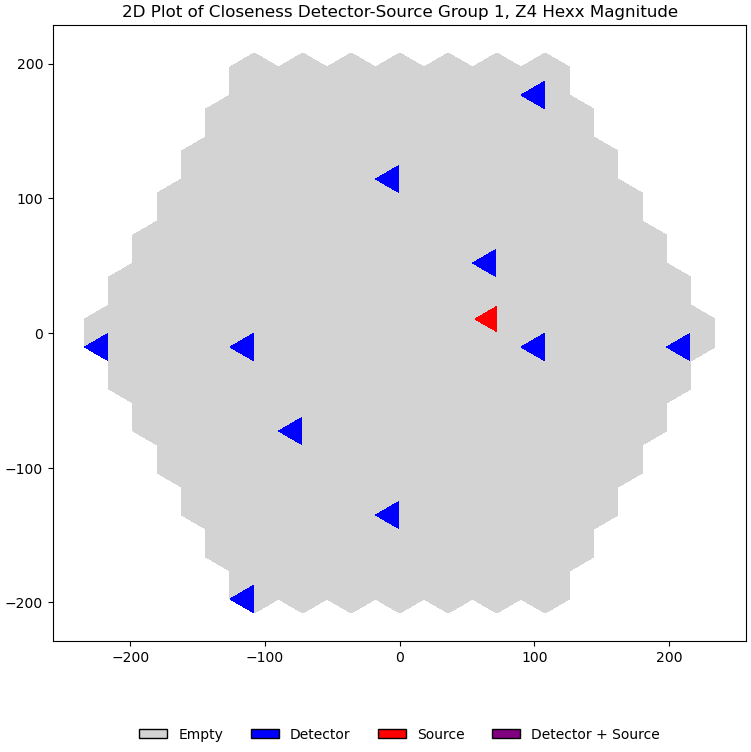
\includegraphics[width=\linewidth]{figures/OBJECTIVES45_TEST15_3DTriMG_HTTR_AVS2S_level1_closeness_det_S_categorical_G1_Z4.png}
        \end{subfigure}
        \hfill
        \begin{subfigure}{.48\textwidth}
          \centering
          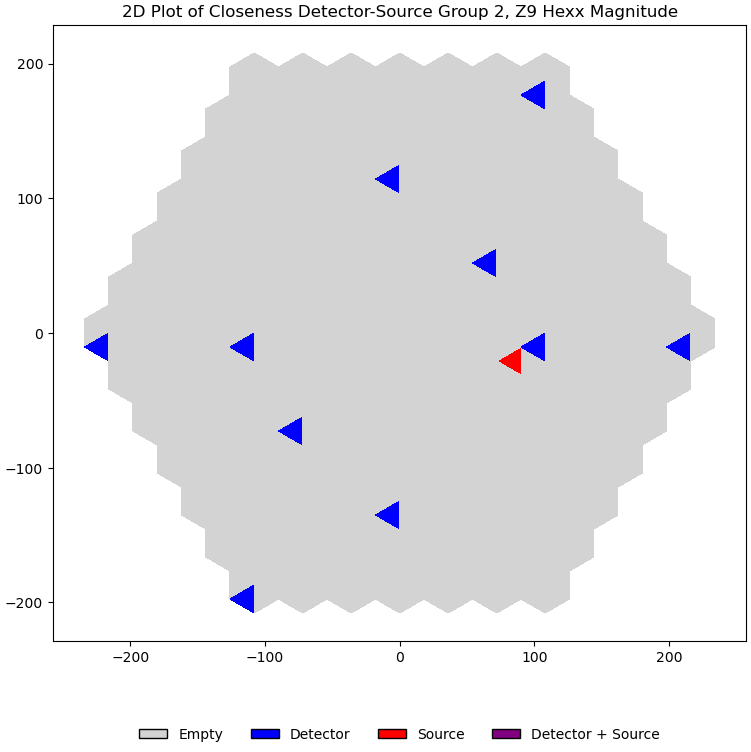
\includegraphics[width=\linewidth]{figures/OBJECTIVES45_TEST15_3DTriMG_HTTR_AVS2S_level1_closeness_det_S_categorical_G2_Z9.png}
        \end{subfigure}
        \caption{Location of source and detectors in the 3D HTTR two sources case}
        \label{fig:map_S_3DHTTR_AVS2S}
\end{figure}

The results of the simulations are described in Table \ref{table:unfold_3DHTTR_AVS2S}.
\begin{table}[H]
        \centering
        \caption{Two noise sources in 3D HTTR}
        \label{table:unfold_3DHTTR_AVS2S}
        \begin{tabular}{ | M{2cm} | M{1.5cm} | M{1.5cm} | M{1.5cm} | M{4.5cm} | M{1.5cm} | } 
         \hline
         \textbf{Method} & \textbf{Energy Group} & \textbf{Axial Level} & \textbf{Hex Number} & \textbf{Neutron Noise Source} ($n/cm^3$) & \textbf{Match?}  \\
         \hline
         \multirow{2}{*}{Reference} & 1 & 4 & 66 & $-2.922 \times 10^{-7} + 0.000i$ & -- \\
         \cline{2-6}                & 2 & 9 & 54 & $-3.152 \times 10^{-8} + 0.000i$ & -- \\
         \hline
         \multirow{2}{*}{Inversion} & 1 & 1 & 1 & $0.000 + 0.000i$ & No \\
         \cline{2-6}                & 1 & 1 & 2 & $0.000 + 0.000i$ & No \\
         \hline
         \multirow{2}{*}{Zoning} & 2 & 3 & 9 & $-1.395 \times 10^{-7} + 1.386 \times 10^{-7}i$ & No \\
         \cline{2-6}             & 2 & 3 & 3 & $-1.147 \times 10^{-7} + 1.105 \times 10^{-7}i$ & No \\
         \hline
         \multirow{2}{*}{Scanning} & 2 & 2 & 66 & $-2.423 \times 10^{-7} - 1.078 \times 10^{-9}i$ & No \\
         \cline{2-6}               & 1 & 4 & 1 & $0.000 + 0.000i$ & No \\
         \hline
         \multirow{2}{*}{Brute Force} & 1 & 4 & 66 & $-2.922 \times 10^{-7} + 0.000i$ & Yes \\
         \cline{2-6}                  & 2 & 9 & 54 & $-3.152 \times 10^{-8} + 0.000i$ & Yes \\
         \hline
         \multirow{2}{*}{Greedy} & 1 & 4 & 66 & $-2.922 \times 10^{-7} + 0.000i$ & Yes \\
         \cline{2-6}             & 2 & 9 & 54 & $-3.152 \times 10^{-8} + 0.000i$ & Yes \\
         \hline
        \end{tabular}
\end{table}
Similar to the two-mesh source of the 2D HTTR case, the results show that the inversion, zoning, and scanning method fail to unfold the neutron noise source. The inversion and zoning method is expected to fail, since it fails in a single source. The scanning method fails due to the method’s limitation, as it only points to one location that minimizes the ratio difference (see Eq. \ref{eq:scan_min}). On the other hand, brute force and greedy methods manage to unfold the neutron noise source. This is expected behavior for both methods.

\subsubsection{Three Mesh Source}

In this simulation, a three-mesh AVS source is unfolded using both the existing and novel methods. The simulation is done with a constant frequency of 1 Hz. There are 21 detectors in this case. Each detector can accurately detect neutron noise for the whole fuel column. The noise source is located in two different groups and axial levels. The first source is located at $Z=1$ (top of the core) and fast group, the second source is located at $Z=5$ (midplane) in thermal group, and the third source is located at $Z=9$ (bottom of the core) in thermal group. Figure \ref{fig:map_S_3DHTTR_AVS3S} shows the location of the AVS source.
\begin{figure}[H]
        \centering
        \begin{subfigure}{.48\textwidth}
          \centering
          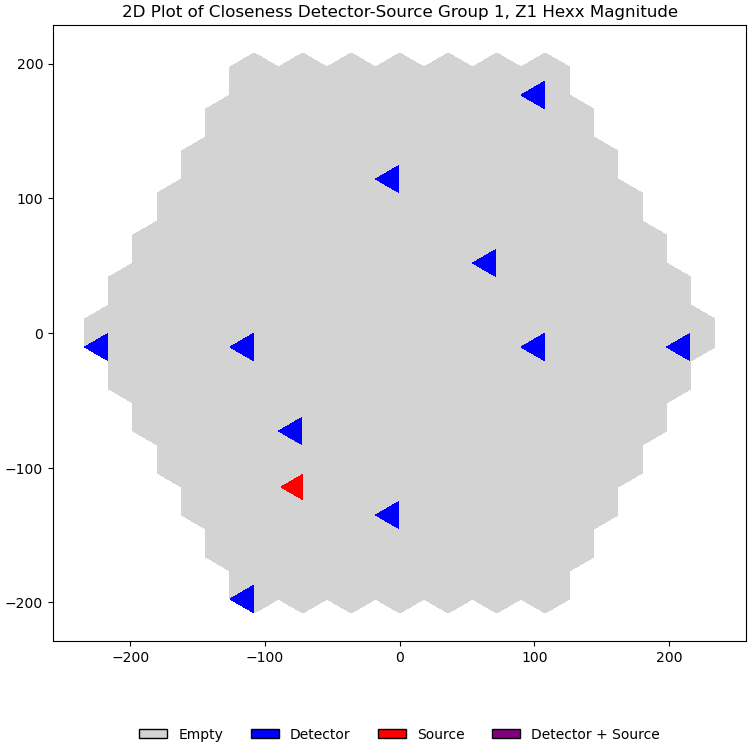
\includegraphics[width=\linewidth]{figures/OBJECTIVES45_TEST12_3DTriMG_HTTR_AVS3S_level1_closeness_det_S_categorical_G1_Z1.png}
        \end{subfigure}
        \hfill
        \begin{subfigure}{.48\textwidth}
          \centering
          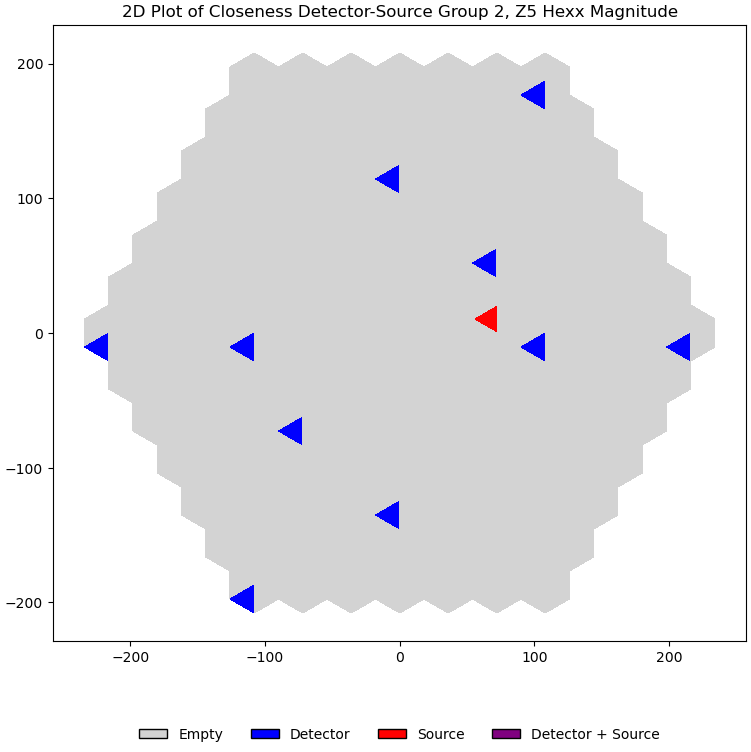
\includegraphics[width=\linewidth]{figures/OBJECTIVES45_TEST12_3DTriMG_HTTR_AVS3S_level1_closeness_det_S_categorical_G2_Z5.png}
        \end{subfigure}
        \hfill
        \begin{subfigure}{.48\textwidth}
          \centering
          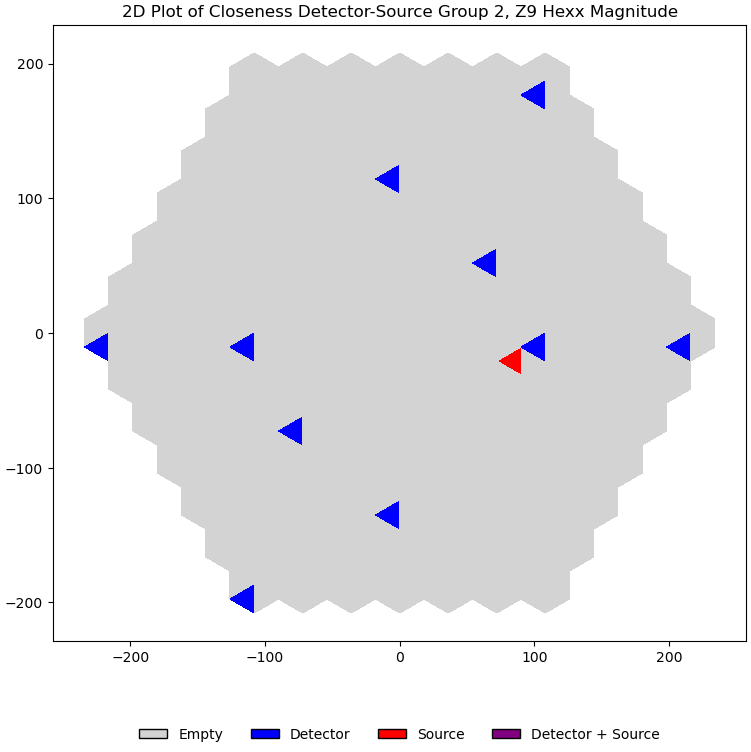
\includegraphics[width=\linewidth]{figures/OBJECTIVES45_TEST12_3DTriMG_HTTR_AVS3S_level1_closeness_det_S_categorical_G2_Z9.png}
        \end{subfigure}
        \caption{Location of source and detectors in the 3D HTTR three sources case}
        \label{fig:map_S_3DHTTR_AVS3S}
\end{figure}

The results of the simulations are described in Table \ref{table:unfold_3DHTTR_AVS3S}.
\begin{table}[H]
        \centering
        \caption{Three noise source in 3D HTTR}
        \label{table:unfold_3DHTTR_AVS3S}
        \begin{tabular}{ | M{2cm} | M{1.5cm} | M{1.5cm} | M{1.5cm} | M{4.5cm} | M{1.5cm} | } 
         \hline
         \textbf{Method} & \textbf{Energy Group} & \textbf{Axial Level} & \textbf{Hex Number} & \textbf{Neutron Noise Source} ($n/cm^3$) & \textbf{Match?}  \\
         \hline
         \multirow{2}{*}{Reference} & 1 & 1 & 18 & $-3.696 \times 10^{-10} + 0.000i$ & -- \\
         \cline{2-6}                & 2 & 5 & 66 & $-4.912 \times 10^{-6} + 0.000i$ & -- \\
         \cline{2-6}                & 2 & 9 & 54 & $-3.152 \times 10^{-8} + 0.000i$ & -- \\
         \hline
         \multirow{2}{*}{Inversion} & 1 & 1 & 1 & $0.000 + 0.000i$ & No \\
         \cline{2-6}                & 2 & 1 & 1 & $0.000 + 0.000i$ & No \\
         \cline{2-6}                & 2 & 1 & 2 & $0.000 + 0.000i$ & No \\
         \hline
         \multirow{2}{*}{Zoning} & 2 & 3 & 9 & $-3.339 \times 10^{-6} + 2.604 \times 10^{-6}i$ & No \\
         \cline{2-6}             & 2 & 3 & 3 & $-4.912 \times 10^{-6} + 2.078 \times 10^{-6}i$ & No \\
         \cline{2-6}             & 2 & 2 & 90 & $-3.152 \times 10^{-6} + 1.829 \times 10^{-6}i$  & No \\
         \hline
         \multirow{2}{*}{Scanning} & 2 & 2 & 66 & $-4.922 \times 10^{-6} - 1.243 \times 10^{-8}i$ & No \\
         \cline{2-6}               & 1 & 4 & 1 & $0.000 + 0.000i$ & No \\
         \cline{2-6}               & 1 & 4 & 2 & $0.000 + 0.000i$ & No \\
         \hline
         \multirow{2}{*}{Brute Force} & 1 & 1 & 18 & $-3.696 \times 10^{-10} + 0.000i$ & Yes \\
         \cline{2-6}                  & 2 & 5 & 66 & $-4.912 \times 10^{-6} + 0.000i$ & Yes \\
         \cline{2-6}                  & 2 & 9 & 54 & $-3.152 \times 10^{-8} + 0.000i$ & Yes \\
         \hline
         \multirow{2}{*}{Greedy} & 1 & 1 & 18 & $-3.696 \times 10^{-10} + 0.000i$ & Yes \\
         \cline{2-6}             & 2 & 5 & 66 & $-4.912 \times 10^{-6} + 0.000i$ & Yes \\
         \cline{2-6}             & 2 & 9 & 54 & $-3.152 \times 10^{-8} + 0.000i$ & Yes \\
         \hline
        \end{tabular}
\end{table}
Similar to the three-mesh source of 2D HTTR results, the results show that the inversion, zoning, and scanning method fails to unfold the neutron noise source. On the other hand, brute force and greedy methods are able to unfold the neutron noise source. This is expected behavior for both methods.

\section{Limitation of Novel Methods}

\subsection{Limitation of Brute Force Method}

The main limitation of the brute force method is the time necessary to calculate all combinations of Green’s function. Since the brute force iterates the process serially, the cost of the calculation grows exponentially. For example, the discretization used for 2D problem is relatively coarse. It solves for 1524 unknowns (2 groups x 762 mesh). Table \ref{table:brute_comb_number} shows the number of combinations that need to be solved in the brute force method for 2D HTTR. 
\begin{table}[H]
        \centering
        \caption{Number of combinations to solve in brute force method}
        \label{table:brute_comb_number}
        \begin{tabular}{ | M{2cm} | M{3cm} | } 
         \hline
         \textbf{Number of Sources} & \textbf{Number of Combinations} \\
         \hline
         1 & 1524 \\
         2 & 1.16 $\times 10^{6}$ \\
         3 & 5.89 $\times 10^{8}$ \\
         4 & 2.24 $\times 10^{11}$ \\
         \hline
        \end{tabular}
\end{table}
This makes the use of the brute force method computationally extremely expensive when the number of sources exceeds two.

\subsection{Limitation of Greedy Method}
\label{sec:greedy_limit}

The greedy method performs two iterations. The first iteration involves searching for a list of valid solutions by identifying the Green’s function component that leads to a local minimum residual. The second iteration aims to find a solution for the list of valid solutions that minimizes the residual within a certain tolerance and has the least amount of Green’s function components. It should be noted that residual in this case is the residual between the Green’s function combination and the measured neutron noise.

The quality and availability of the measured neutron noise data limit the performance of the greedy method. With a limited amount of measured neutron noise data, it would be possible to have an unfolding solution that is only partially correct (identifies some, but not all noise courses). This is because with limited measured neutron noise data, the residual calculation becomes under-constrained, meaning the greedy method may require more combinations of Green’s functions to reach the desired residual. Table \ref{table:greedy_source} shows the matching results for the greedy method applied to 2D HTTR for an increasing number of noise sources. The 2D HTTR core used in this case has 21 detectors, which means there are only 21 measured neutron noise data points. In these simulations, for each number of sources, the unfolding is repeated up to 10 times with different combinations of frequencies, magnitudes, energies, and locations. The sample values for these simulations are provided in Appendix \ref{ch:appendixC}. A similar simulation is done with 30 detectors to show the effect of availability of measured neutron noise data.
\begin{table}[H]
        \centering
        \caption{Reliability of greedy method with varying number of sources}
        \label{table:greedy_source}
        \begin{tabular}{ | M{2cm} | M{2.5cm} | M{2.5cm} |  M{2.5cm} | } 
         \hline
         \multirow{2}{=}{\centering\textbf{Number of Sources}} & 
         \multicolumn{2}{c|}{\textbf{Match Percentage}} \\ 
         \cline{2-3}
         &\textbf{21 Detectors} & \textbf{30 Detectors} \\
         \hline
         1 & 100\% & 100\% \\
         2 & 100\% & 100\% \\
         3 & 100\% & 100\% \\
         4 & 100\% & 100\% \\
         5 & 100\% & 100\% \\
         6 & 100\% & 100\% \\
         7 & 50\%  & 100\% \\
         \hline
        \end{tabular}
\end{table}

Table \ref{table:greedy_source} shows that with 21 measured neutron noise data, the greedy method can be reliable up to six noise sources. At seven noise sources, the greedy method becomes unreliable. However, using 30 measured neutron noise data, the reliability of the greedy method for seven noise sources is improved.

\section{Conclusion}

This chapter reviews the existing neutron noise unfolding methods and introduces novel methods that utilize Green’s function. The novel methods are the brute force method and the greedy method. The development of new methods is necessary, considering the limitations of the existing methods. The brute force method iterates through all combinations of Green’s function until it finds the combination that minimizes the residual below a certain tolerance. The greedy method is inspired by the matching pursuit algorithm in compressed sensing. In every iteration, it looks for the Green’s function component that minimizes the residual. This results in several valid solutions that overfit the residual. In the second step, the greedy method seeks a combination of Green’s functions from the valid solutions with the least number of components. 

Both the existing methods and the novel methods are applied to unfold neutron noise sources in the 2D HTTR and 3D HTTR core. The noise sources are defined as AVS-type sources. The unfolding is done using multiple AVS-type sources. The results show that the inversion and zoning methods are not reliable for unfolding neutron noise in HTTR. The scanning method is able to unfold only single neutron noise source and is unreliable for unfolding two or more sources. The brute force and greedy methods are effective in unfolding the neutron noise in the 2D and 3D HTTR core for at least 3 noise sources.